\subsection{LHC New Physics Dataset}
{{\footnotesize
\noindent A dataset of proton-proton collision events emulating a 40 MHz real-time data stream from LHC detectors, pre-filtered on electron or muon presence. Designed for unsupervised new-physics detection algorithms under latency/bandwidth constraints.


\begin{description}[labelwidth=4cm, labelsep=1em, leftmargin=4cm, itemsep=0.1em, parsep=0em]
  \item[date:] 2021-07-05
  \item[version:] v1.0
  \item[last\_updated:] 2021-07
  \item[expired:] unknown
  \item[valid:] yes
  \item[valid\_date:] 2021-07-05
  \item[url:] \href{https://arxiv.org/pdf/2107.02157}{https://arxiv.org/pdf/2107.02157}
  \item[doi:] unknown
  \item[domain:] Particle Physics; Real-time Triggering
  \item[focus:] Real-time LHC event filtering for anomaly detection using proton collision data
  \item[keywords:]
    - anomaly detection
    - proton collision
    - real-time inference
    - event filtering
    - unsupervised ML
  \item[licensing:] unknown
  \item[task\_types:]
    - Anomaly detection
    - Event classification
  \item[ai\_capability\_measured:]
    - Unsupervised signal detection under latency and bandwidth constraints
  \item[metrics:]
    - ROC-AUC
    - Detection efficiency
  \item[models:]
    - Autoencoder
    - Variational autoencoder
    - Isolation forest
  \item[ml\_motif:]
    - Multiple
  \item[type:] Framework
  \item[ml\_task:]
    - NA
  \item[solutions:] 0
  \item[notes:] Includes electron/muon-filtered background and black-box signal benchmarks; 1M events per black box.

  \item[contact.name:] Ema Puljak (ema.puljak@cern.ch)
  \item[contact.email:] unknown
  \item[datasets.links.name:] Zenodo stores, background + 3 black-box signal sets. 1M events each
  \item[results.links.name:] ChatGPT LLM
  \item[fair.reproducible:] Yes
  \item[fair.benchmark\_ready:] Yes
  \item[id:] lhc\_new\_physics\_dataset
  \item[Citations:] \cite{https://doi.org/10.5281/zenodo.5046389}
\end{description}

{\bf Ratings:} ~ \\

\begin{tabular}{p{0.15\textwidth} p{0.07\textwidth} p{0.7\textwidth}}
\hline
Rating & Value & Reason \\
\hline
dataset & 5 & Large-scale dataset hosted on Zenodo, publicly available, well-documented, with defined train/test structure.
Appears to follow at least 4 FAIR principles.
 \\
documentation & 3 & Some description in papers and dataset metadata exists, but lacks a unified guide, README,
or training setup in a central location.
 \\
metrics & 4 & Uses reasonable metrics (ROC-AUC, detection efficiency) that capture performance but lacks
full explanation and standard evaluation tools.
 \\
reference\_solution & 2 & Baselines are described across multiple papers but lack centralized, reproducible implementations
and hardware/software setup details.
 \\
software & 3 & While not formally evaluated in the previous version, Zenodo and paper links suggest available code for baseline models
(e.g., autoencoders, GANs), though they are scattered and not unified in a single repository.
 \\
specification & 3 & The task and context are clearly described, but system constraints and formal inputs/outputs are not fully specified.
 \\
\hline
\end{tabular}

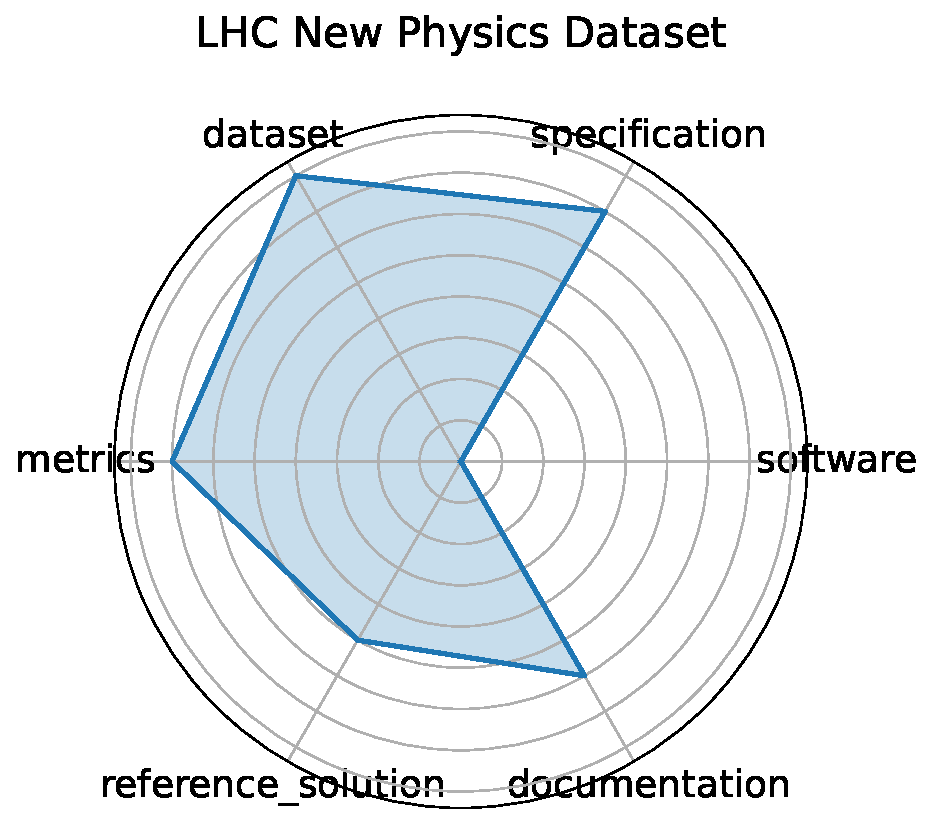
\includegraphics[width=0.2\textwidth]{lhc_new_physics_dataset_radar.pdf}
}}
\clearpage